\pdfminorversion 7
\pdfobjcompresslevel 3

\PassOptionsToPackage{table}{xcolor}
\documentclass[10pt,a4paper]{article}
%\documentclass[10pt,oneside,noprintercorrection]{article}
\special{papersize=210mm,297mm}


\usepackage[absolute]{textpos} 
\usepackage{pdfpages}
\usepackage[utf8]{inputenc}
\usepackage[T1]{fontenc}
\usepackage{cite}
\usepackage[francais]{babel}
\usepackage[bookmarks=false,colorlinks,linkcolor=blue]{hyperref}
\usepackage[top=4cm,bottom=3cm,left=3cm,right=3cm]{geometry}
\usepackage{graphicx}
\usepackage{wrapfig}
\usepackage{subfig}
\usepackage{eso-pic}
\usepackage{array}
\usepackage{listings}
\usepackage{color}
\usepackage[table]{xcolor}
\usepackage{url}
\usepackage{eurosym}
\usepackage{url}
\usepackage{textcomp}
\usepackage{fancyhdr} 
\usepackage{amsmath}
\usepackage{pict2e}
\usepackage{listings}
\usepackage{setspace}
\usepackage{float}
\usepackage[ruled,vlined,linesnumbered]{algorithm2e}
\usepackage[toc,page]{appendix} 
\onehalfspacing
\lstset{escapeinside={<@}{@>}}
\definecolor{lightgray}{gray}{0.9}


\title{Kmer signature in mitochondrial genomes for metagenome taxonomic assignation}

\author{J\'er\'my Fontaine and Samuel Blanquart}


\begin{document}
\maketitle

\section{Semaine 1: Mardi 2 Juillet}

\subsection{R\'eduction de la BDD}
~\\

La base de donnée complète totalise \textbf{30Go}, l'objectif était de réduire la taille de cette BDD en n'ayant les données qu'aux feuilles, pour les autres noeuds de l'arbre les données sont sous forme de lien symbolique. On obtient au final une BDD avec une taille de \textbf{1,1GO}.
~\\

Pour cela:
\\
\begin{itemize}
 \item Modification du fichier chemin-liste d’accession (voir figure \ref{resultatS})
  \item Script de remplissage des noeuds internes
\end{itemize}
~\\

\begin{figure}[H]
\begin{center}
\begin{tabular}{*{2}{c}}
  tax1/tax2/.../taxonFeuilleX : & accession\_1,...,accession\_N  \\
  tax1/tax2/.../taxonFeuilleY : & accession\_1,...,accession\_M  \\
\end{tabular}
\caption{\label{resultatS} Exemple de fichier "chemin: liste d'accession"}
\end{center}
\end{figure}
~\\

L'idée pour générer les liens symboliques est de faire remonter chaque données feuilles vers la racine de la BDD (figure \ref{linkage}).

\lstset{
	language=C,
	morecomment=[l][keywordstyle]{@\#},
	keywordstyle=\bfseries\ttfamily\color[rgb]{0,0,1},
	identifierstyle=\ttfamily,
	commentstyle=\color[rgb]{0.133,0.545,0.133},
	stringstyle=\ttfamily\color[rgb]{0.627,0.126,0.941},
	showstringspaces=false,
	basicstyle=\small,
	numberstyle=\footnotesize,
	numbers=left,
	stepnumber=1,
	numbersep=8pt,
	tabsize=2,
	breaklines=true,
	prebreak = \raisebox{0ex}[0ex][0ex]{\ensuremath{\hookleftarrow}},
	breakatwhitespace=false,
	aboveskip={1.5\baselineskip},
  columns=fixed,
  upquote=true,
  extendedchars=true,
  frame=single,
% backgroundcolor=\color{
}

\begin{figure}[H]
  

\begin{lstlisting}[numbers=left][caption=test]
      //
Pour chaque feuille l de la BBD
{
    /* On se deplace au niveau de la feuille */
    cd l;
    Pour chaque fichier f du dossier courant;
    {
      /* on se deplace dans la parent de cette feuille */  
      courant = pwd // commande unix
      tant que courant != racine
      {
        ln -s X
        /* on remonte d'un niveau */
        cd .. ;
        courant = pwd
      }
      /* on se replace a la feuille pour traiter le nouveau fichier */
      cd l;
    }
}                                            
\end{lstlisting}
\caption{\label{linkage} Algo lien symbolique}
\end{figure}
~\\

\subsection{Krona}
  krona est un utilitaire qui permet de visualiser des hiérarchies sous forme de camembert "zoomables". Pour cela cette hiérarchies doit être écrites sous formes de fichier xml. Krona construit ensuite un fichier html local, un navigateur web permet alors de visualiser le camembert. (figure \ref{krona})
  
  \begin{figure}[H]
\begin{lstlisting}[numbers=left][caption=test]
<node name="Alveolata">
    <genomes><val>1009</val></genomes>
    
    <node name="Apicomplexa">
        <genomes><val>993</val></genomes>
        ...
    </node>      
</node>                                          
\end{lstlisting}
\caption{\label{krona}Exemple simplifié d'un fichier pour krona}
\end{figure}
~\\

\subsection{Scripts dmp et krona}
  En fin de semaine, deux scripts ont été développés pour: 
  \begin{itemize}
    \item Récupérer/mettre à jour les fichiers dmp pour la construction de la bdd.
    \item Récupérer et installer krona
  \end{itemize}

\newpage
\section{Semaine 2: Lundi 7 Juillet}

\subsection{Générer le fichier weka à partir d'un dossier}
  L'idée première était de générer le fichier de comptage au format weka à partir d'un dossier. Pour se faire pour un dossier $D$ il faut effectuer le comptage pour ses sous dossier $d_1,...,d_n$ en prenant soins de récupérer chaque taxid pour chaque $d_i$ afin de lancer le programme de comptage {\textit{count\_kmer} avec les bons arguments. Le programme a était réalisé en Perl.\\ (trunk$/$generate\_learn$/$generate\_learn.pl)
  
  \subsubsection{Parallélisme}
  Au lieu de lancer le programme réalisé auparavant il est possible à partir des options d'utiliser plusieurs processeurs afin d'effectuer plusieurs comptage. Cependant même si le programme offre cette fonctionnalité lors de l'appel system de Perl pour appeler le programme C de comptage, Perl rend immédiatement la main et lance l'appel système suivant, le parallélisme se fait alors par défaut.
  
\subsection{Générer les fréquences de kmer aux feuilles}
  Le but de cette partie est de générer les fréquences uniquement aux feuilles. Ainsi pour construire le fichier weka à un noeud donnée $d$ il suffit d'aller récupérer les fréquences aux feuilles du sous arbre ayant pour pour racine $d$.  (trunk$/$generate\_learn$/$generate\_count.pl)
  

\newpage
\section{Semaine 3: Mardi 15 Juillet}


\subsection{Gestion d'erreur en C}
  Une partie de cette semaine a été consacrée au débogage du comptage écrit en C. En effet le comptage à la racine avec une fenêtre de 50, provoquait des erreurs 
  d'allocation mémoire. Ce problème fut régler grâce à la re-allocation de la mémoire. 
  \subsection{Taille du jeu de fréquences à la racine}
  Avec une taille de fenêtre glissante constante, la taille du fichier de fréquence est proportionnel à la somme des tailles de séquences (nombre de nucléotides totale). On a pu évaluer ainsi la taille du fichier de fréquence au plus haut niveau avec une fenêtre de taille 50 et le pattern \#\#\#\#. On obtiendrai au niveau de la racine, une taille de \textbf{123Go} pour le fichier de fréquence et un temps de \textbf{120 min}. Ainsi grâce aux graphes ci dessous on a pu évaluer le temps (fig. \ref{temps_cpt}) pour générer le fichier de fréquence et la taille de celui-ci (fig. \ref{taille_cpt}) sur l'ensemble des séquences (251 371 097 nucléotides).
  
  
\begin{figure}[H]
\begin{center}
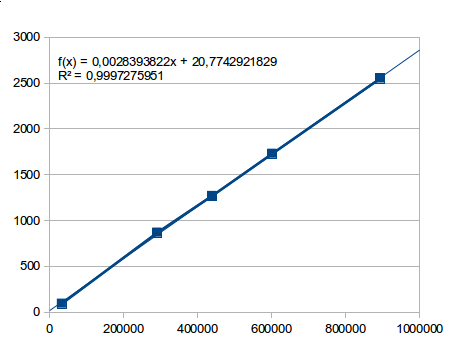
\includegraphics[scale=0.6]{./../img/graphe_temps.png}
\caption[Temps de du comptage]{\label{temps_cpt}Temps en seconde en fonction de la taille de la séquence avec une fenêtre de taille 50}
\end{center}
\end{figure}

\begin{figure}[H]
\begin{center}
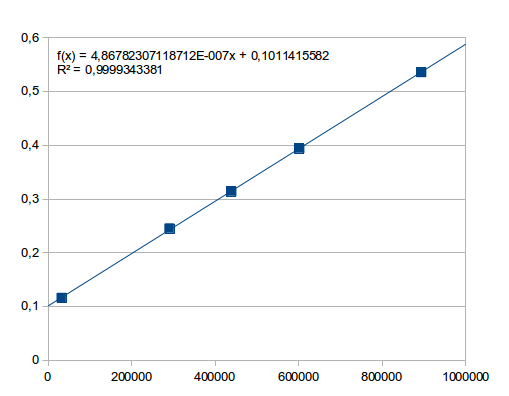
\includegraphics[scale=0.6]{./../img/graphe_taille.png}
\caption[Temps de du comptage]{\label{taille_cpt}Temps en seconde en fonction de la taille de la séquence avec une fenêtre de taille 50}
\end{center}
\end{figure}
  
\subsection{Passage aux objets}
Pour la suite du projet on décide de passer au c++ afin de tout gérer en tant qu'objet, on pourra ainsi plus aisément manipuler la table de fréquence en kmers. La génération
de données pour weka, la validation croisée...
\subsubsection{Les classes}
Pour le moment on ne manipule que trois classes:
\begin{itemize}
 \item classData: pour gérer les données (séquences,taille, nombre de jeux de données, responsable du comptage)
  \item classPattern: gestion d'un kmer
  \item FreqKmer: classe principale gérant principalement le tableau de fréquence.
\end{itemize}
~\\

L'objet à la possibilité de s'instancier à partir 
\begin{itemize}
 \item[.] D'un fichier fasta
 \item[.] D'un fichier contenant une liste de chemins vers des fichiers fasta.
\end{itemize}
~\\

De ce fait lorsqu'on souhaite obtenir la fréquence à un niveau, c'est au niveau des feuilles du sous arbre définit par ce niveau où l'on va effectuer le comptage.

En fin de semaine des tests de validation ont été rajoutés au programme. 


%commentaire

\end{document}



